\documentclass{report}
\usepackage{listings}
\usepackage{hyperref}
\usepackage{tikz}
\usetikzlibrary{shapes.geometric, arrows}
\tikzstyle{process} = [rectangle, minimum width=3cm, minimum height=1cm, text centered, text width=6cm, draw=black]
\tikzstyle{arrow} = [thick,->,>=stealth]

\begin{document}

\title{Tastydoc: a cocumentation tool for dotty using Tasty files}
\author{Bryan Abate
\\\\\small{Supervised by Aleksander Boruch-Gruszecki}}

\maketitle

\begin{abstract}
The current documentation tool (dottydoc) relies on compiler internals and low level code. The tool introduced here aims to build a program not dependant on compiler internals but instead use Tasty files which are output when a Scala program is compiled.

It also aims at providing a tool with less bugs, more features and which is more easily maintenable.

For flexibility the output is in Markdown instead of the commonly used HTML.
\end{abstract}

\tableofcontents

\chapter{Introduction}
In dotty the documentation generation tool is called \texttt{dotty-doc}. However the tool is flawed in many ways, these flaws include:
\begin{itemize}
    \item Reliance on compiler internals
    \item Low level and unecessarily complex code which make it hard to maintain
    \item Not maintened and not documented
    \item Not flexible in its output, it outputs HTML/css in a hard to modify way
    \item Malformed type output such as \texttt{[32m"getOffset"[0m}
    \item Classes often show to be extending Object instead of their superclass. Example: \url{https://dotty.epfl.ch/api/scala/Conversion.HTML}
\begin{lstlisting}[language=scala]
abstract class Conversion [ -T, +U ] extends Object with Function1
\end{lstlisting}
    \item Annotations which sould not be display, sometimes are. Example:
    \item Lacks some features, especially:
    \begin{itemize}
        \item No known subclasses
        \item 
    \end{itemize}
\end{itemize}

The tool introduced here aims to address all these issues while providing with a code easy to maintain and easy to adapt to every need.

One major difference with currrent documentation tools is that the output is in Markdown instead of HTML, this has some pros and cons which will be discussed below.

Althought dotty-doc has some problems, the current tool will draw inspiration for some of its architecture which will allow for its parsing code for user documentation (modified to handle this structure and output Markdown) to be reused.

The report will follow the structure described in this introduction and will conclude with problems of the current implementation and further work.

\chapter{Features}

\chapter{Output format}
Before describing the output, we list the reasons, pros and cons of using a Markdown output.

\section{Reasoning behind Markdown}

The major reason to use Markdown instead of HTML is to think of the documentation tool as a pipeline which would look like this:

\begin{center}
    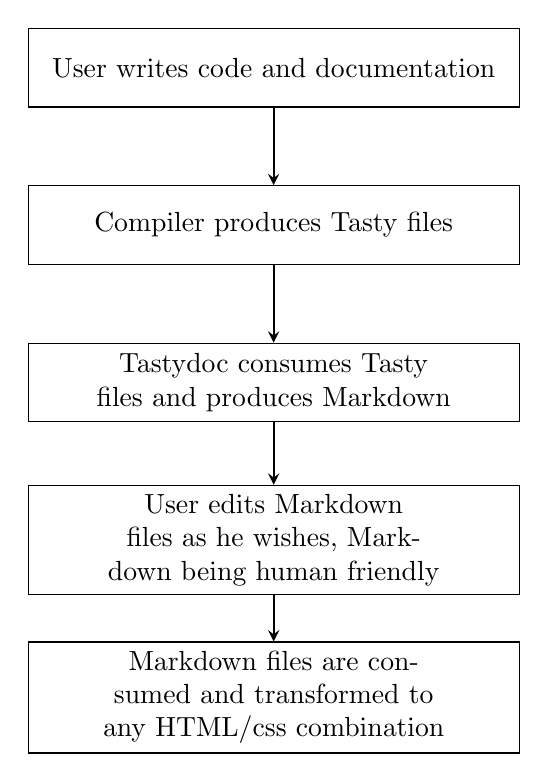
\begin{tikzpicture}[node distance=2cm]
        \node (write) [process] {User writes code and documentation};
        \node (compile) [process, below of=write] {Compiler produces Tasty files};
        \node (tool) [process, below of=compile] {Tastydoc consumes Tasty files and produces Markdown};
        \node (user) [process, below of=tool] {User edits Markdown files as he wishes, Markdown being human friendly};
        \node (HTML) [process, below of=user] {Markdown files are consumed and transformed to any HTML/css combination};
    
        \draw [arrow] (write) -- (compile);
        \draw [arrow] (compile) -- (tool);
        \draw [arrow] (tool) -- (user);
        \draw [arrow] (user) -- (HTML);
    \end{tikzpicture}
\end{center}

With such a pipeline we do not limit the user to use a specific output for the documentation, he can easily remove, add parts, etc. manually and then use an HTML format of his choosing as Markdown only specify the structure not how it should be displayed.

\section{Pros and Cons}

Using Markdown as an intermediate output format comes with some pros and cons comparing to an HTML output:
\begin{itemize}
    \item \textbf{Pros:}
    \begin{itemize}
        \item Human readable and editable, meaning part of the documentation can be written manually
        \item Easy to infer the format of the output to extend it manually
        \item Live preview and editing
        \item Only define the structure of the output not how to display it
        \item Easily pipelined to another format (HTML, reStructuredText, etc.)
    \end{itemize}
    \item \textbf{Cons:}
    \begin{itemize}
        \item No Scala (or Java) library available to output markdown with escaping
        \item Markdown fenced code block cannot contain links which forces us to use html code block, hence loose syntax highlight in Markdown and not output "pure" Markdown.
        \item Markdown does not have "division" like \texttt{<div>} in HTML to better structure the output
    \end{itemize}
\end{itemize}

\section{Output structure}
In the following section, we describe how the markdown output is structured.

\subsection{class, object and trait}
Have their own \texttt{.md} file.

\begin{enumerate}
    \item Name (header 1)
    \item Companion object (header 2)
    \item Signature (HTML pre + code)
    \item User documentation
    \item Annotations (header 2)
    \item Known subclasses (header 2)
    \item Constructors (header 2)
    \begin{enumerate}
        \item Name + paremeters (HTML pre + code)
        \item User documentation
    \end{enumerate}
    \item Members (header 2) (In order: Abstract Type Members, Concrete Type Members, Abstract Value Members, Concrete Value Members)
    \begin{enumerate}
        \item Follows structure described in \autoref{sec:signatureSec}
    \end{enumerate}
\end{enumerate}

\subsection{Package}
Has its own \texttt{.md} file.

\begin{enumerate}
    \item Name (header 1)
    \item Members (header 2)
    \begin{enumerate}
        \item Follows structure described in \autoref{sec:signatureSec} and \autoref{sec:packageSignatureSec}
    \end{enumerate}
\end{enumerate}

\subsection{Type alias, class (simplified format), def, val and var}
No \texttt{.md} file.

\label{sec:signatureSec}
\begin{enumerate}
    \item Name (header 3)
    \item Annotations + signature (HTML pre + code)
    \item User documentation
\end{enumerate}

\subsection{Package (simplified format)}
No \texttt{.md} file.

\label{sec:packageSignatureSec}
\begin{enumerate}
    \item name + link (HTML pre + code)
\end{enumerate}

\chapter{Architecture}

\section{Use of dotty-doc parsing}

\chapter{Problems encountered}

\chapter{Further work}

\chapter{Conclusion}

\end{document}